\section{划分树}
划分树是一种来解决区间第 $K$ 大的一种数据结构,其常数、理解难度都要比主席树低很多。同时,划分树紧贴“第 $K$ 大”,所以是一种基于排序的一种数据结构。
\subsection{建树}
划分树的建树比较简单,但是相对于其他树来说比较复杂。
\begin{figure}[htbp]
	\centering
	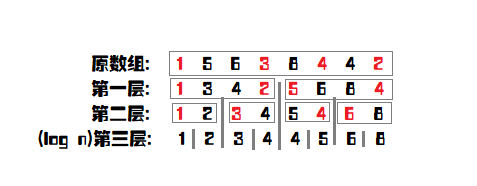
\includegraphics{./image/dividing1.png}
\end{figure}
如图,每一层都有一个看似无序的数组。其实,每一个被红色标记的数字都是 \textbf{要分配到左儿子的} 。而分配的规则是什么?就是与 \textbf{这一层的中位数} 做比较,如果小于等于中位数,则分到左边,否则分到右边。但是这里要注意一下:并不是严格的 \textbf{小于等于就分到左边,否则分到右边}。因为中位数可能有相同,而且与 $N$ 的奇偶有一定关系。下面的代码展示会有一个巧妙的运用,大家可以参照代码。
我们不可能每一次都对每一层排序,这样子不说常数,就算是理论复杂度也过不去。我们想,找中位数,一次排序就够了。为什么?比如,我们求 $[l,r]$ 的中位数,其实就是在排完序过后的 \textit{num[mid]}。
两个关键数组:
tree[log(N),N]:也就是树,要存下所有的值,空间复杂度 $O(n\log n)$。 toleft[log(N),n]:也就是每一层 1~i 进入左儿子的数量,这里需要理解一下,这是一个\textbf{前缀和}。

\subsection{查询}
那我们先扯一下主席树的内容。在用主席树求区间第 $K$ 小的时候,我们以 $K$ 为基准,向左就向左,向右要减去向左的值,在划分树中也是这样子的。

查询难理解的,在于 \textbf{区间缩小} 这种东西。下图,我查询的是 $3$ 到 $7$, 那么下一层我就只需要查询 $2$ 到 $3$ 了。当然,我们定义 $[left, right]$ 为缩小后的区间(目标区间),$[l,r]$ 还是我所在节点的区间。那为什么要标出目标区间呢?因为那是 \textbf{判定答案在左边还是右边的基准}。
\begin{figure}[htbp]
	\centering
	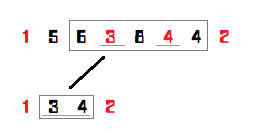
\includegraphics{./image/dividing2.png}
\end{figure}

\subsection{实现}
	\href{http://poj.org/problem?id=2104}{POJ2104 K-th Number} \par 
	$n$ 个数 $m$ 次询问区间 $[l,r]$​ 第 $k$ 小值
	\lstinputlisting{./source/dividing-tree.cpp}
	